\documentclass[9pt]{beamer}

%\usepackage{tikz}
\usepackage{amsmath}
\usepackage{amsfonts}
\usepackage{amssymb}
\usepackage{algorithm2e}
\usepackage{color, colortbl}
\usepackage{enumerate}
\usepackage{arydshln}
\usepackage{multirow}

\renewcommand{\figurename}{Fig}
\usetheme{uha}



%\theoremstyle{plain}
%  \newtheorem{theorem}{Theorem}
%  \newtheorem{lemma}{Lemma}
\newtheorem{corrolary}{Corollary}
\newtheorem{claim}{Claim}
\newtheorem{proposition}{Proposition}
\newtheorem{property}{Property}
%  \newtheorem{fact}{Fact}
%\theoremstyle{definition}
%  \newtheorem{definition}{Definition}
%  \newtheorem{example}{Example}
%\theoremstyle{remark}
\newtheorem{remark}{Remark}
\newtheorem{proviso}{Proviso}


\newcommand{\ccr}[1]{{\color{red}#1}}
\newcommand{\ccb}[1]{{\color{blue}#1}}
\newcommand{\ccp}[1]{{\color{purple}#1}}
\newcommand{\ccm}[1]{{\color{magenta}#1}}
\newcommand{\cco}[1]{{\color{orange}#1}}
\newcommand{\ccy}[1]{{\color{yellow}#1}}
\newcommand{\ccl}[1]{{\color{lime}#1}}
\newcommand{\ccc}[1]{{\color{cyan}#1}}
\newcommand{\ccg}[1]{{\color{gray}#1}}
\newcommand{\ccpk}[1]{{\color{pink}#1}}
\newcommand{\ccov}[1]{{\color{olive}#1}}



\begin{document}

%%//////////////////////////////////////////////////////////////////////////////////////////////%%1

\title{Clustering}
\subtitle{K-means}
\author{Haotian Wang and Yiyan Li}
\institute{School of Software, Shanghai Jiao Tong University}
\date{\hspace{2em}}
\frame{
	\titlepage
}
%%//////////////////////////////////////////////////////////////////////////////////////////////%%
\section{Introduction to clustering}
\begin{frame}
	\frametitle{Clustering}
	\begin{definition}
		A cluster is a collection of objects which are “similar” between them and are “dissimilar” to the objects belonging to other clusters.
	\end{definition}
	\begin{definition}
		Clustering is the algorithm that recognizes clusters from a given data set.
	\end{definition}
	\pause
	Part of common application domains in which the clustering problem arises are as follows:
	\begin{itemize}
		\item Multimedia Data Analysis
		\item Responding to public health crises
		\item Intermediate Step for other fundamental data mining problems
		\item Intelligent Transportation
	\end{itemize}
\end{frame}

%%//////////////////////////////////////////////////////////////////////////////////////////////%%1
\section{K-means Algorithm}
%%//////////////////////////////////////////////////////////////////////////////////////////////%%
\begin{frame}
	\frametitle{K-means}
	The \ccp{k-means clustering} problem is one of the oldest and most important questions in all of computational geometry.
	\par Given an integer $k$ and a set of $n$ data points in $\mathbb{R}^{d}$, the goal of this problem is to choose \ccp{$k$ centers} so as to \ccp{minimize the total squared distance between each point and its closest center}.
	\par The most common K-means algorithm was first proposed by \ccp{Stuart Lloyd} of Bell Labs in 1957.

\end{frame}
%%//////////////////////////////////////////////////////////////////////////////////////////////%%
\begin{frame}
	\frametitle{K-means}
	The objective function to minimize is the \ccp{within-cluster sum of squares} (WCSS) cost:
	$$Cost(C_{1:k}, c_{1:k}) = \sum_{i=1}^{k} \sum_{x \in C_i } {\left\lVert x - c _i \right\rVert }^2  $$
	where $c_i$ is the \ccp{centroid} of cluster
	\begin{definition}
		\ccp{Cluster centroid} is the \ccp{middle} of a cluster.
		\par A centroid is a vector that contains one number for each variable, where each number is the mean of a variable for the observations in that cluster.
		\par The centroid can be thought of as the multi-dimensional average of the cluster.
	\end{definition}
\end{frame}
%%//////////////////////////////////////////////////////////////////////////////////////////////%%
\begin{frame}
	\frametitle{K-means}
	\begin{lemma}
		Let $C$ be a cluster of points with its mean to be $\mu$, and let $c$ to be and arbitrary point.Then $\sum_{x \in C}{\left\lVert x - c\right\rVert}^2 = \sum_{x \in C}{\left\lVert x - \mu\right\rVert}^2 + \left\lvert C \right\rvert \cdot {\left\lVert c - \mu\right\rVert}^2 $
	\end{lemma}
	So we denote that:
	\begin{equation*}
		\begin{split}
			Cost(C_{1:k}, c_{1:k}) & = \sum_{i=1}^{k} \sum_{x \in C_i } {\left\lVert x - c _i \right\rVert }^2 \\
			& = \sum_{i=1}^{k} (\sum_{x \in C_i} {\left\lVert x - \mu_i\right\rVert}^2 + \left\lvert C_i \right\rvert \cdot {\left\lVert c_i - \mu_i\right\rVert}^2) \\
			& = Cost(C_{1:k}, mean(C_{1:k})) + \sum_{i=1}^{k} {\left\lvert C_i\right\rvert }\cdot {\left\lVert c_i - \mu_i\right\rVert }^2
		\end{split}
	\end{equation*}
\end{frame}
%%//////////////////////////////////////////////////////////////////////////////////////////////%%
\begin{frame}
	\frametitle{Toward a K-means Algorithm}
	The k-means algorithm \ccp{iteratively} calculates the sum of distance within a cluster and updates the partition.
	\begin{enumerate}
		\item Arbitrarily choose and initial \ccb{$k$} centroids \ccb{$\mathcal{C} = \{c_1, c_2 \dots c_k\}$}
		\item For each $i \in \{1, 2 \dots k\}$, set the cluster $C_i$ to be the set of points that are \ccp{closer} to $c_i$ than they are to $c_j$ for all $j \neq i$
		\item For each $i \in \{1, 2 \dots k\}$, set $c_i$ to be the center of all points in $C_i$ where \ccb{$c_i = \frac{1}{\left\lvert C_i \right\rvert }\sum_{x \in C_i} x $}
		\item Repeat Step 2 and Step 3 until \ccb{$\mathcal{C}$} no longer changes.
	\end{enumerate}
\end{frame}

\begin{frame}
	\frametitle{Toward a K-means Algorithm}
	Iteration = 1
	\centerline{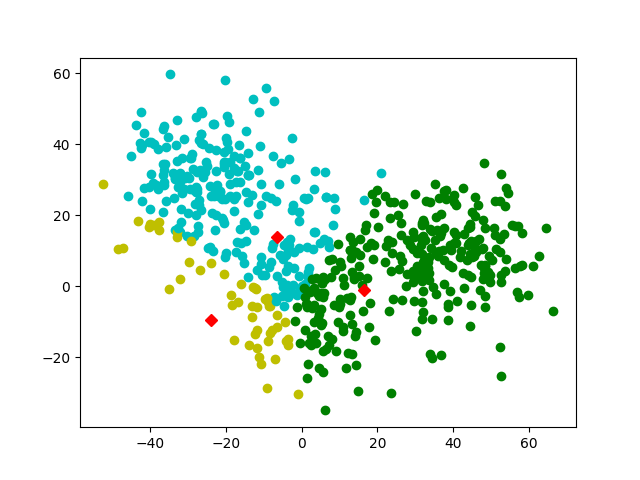
\includegraphics[width=0.65\textwidth]{figures/iteration1.png}}

\end{frame}

\begin{frame}
	\frametitle{Toward a K-means Algorithm}
	Iteration = 2
	\centerline{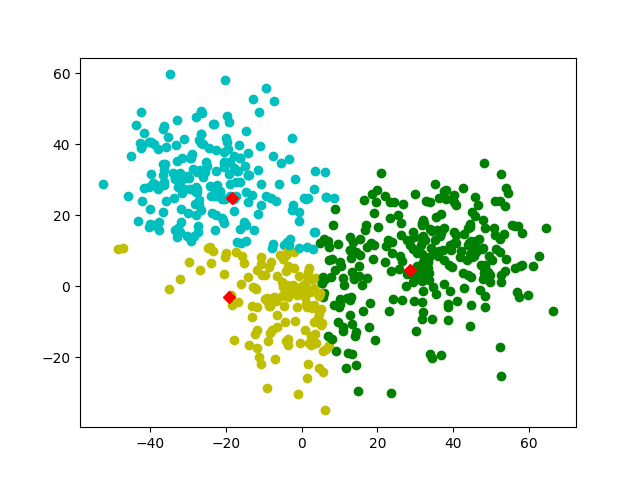
\includegraphics[width=0.65\textwidth]{figures/iteration2.png}}

\end{frame}

\begin{frame}
	\frametitle{Toward a K-means Algorithm}
	Iteration = 3
	\centerline{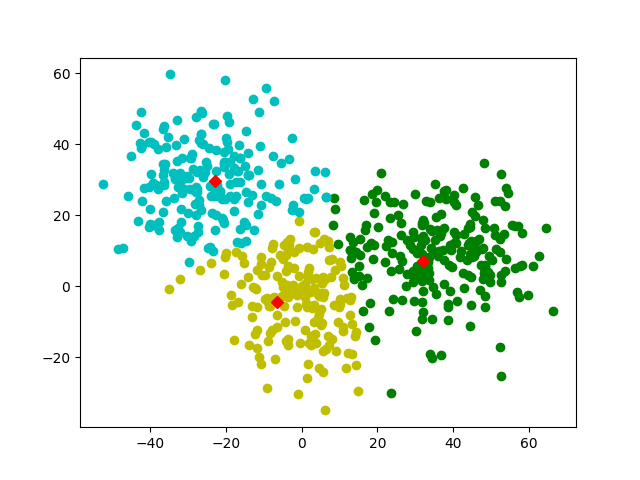
\includegraphics[width=0.65\textwidth]{figures/iteration3.png}}

\end{frame}

\begin{frame}
	\frametitle{Toward a K-means Algorithm}
	Iteration = 4
	\centerline{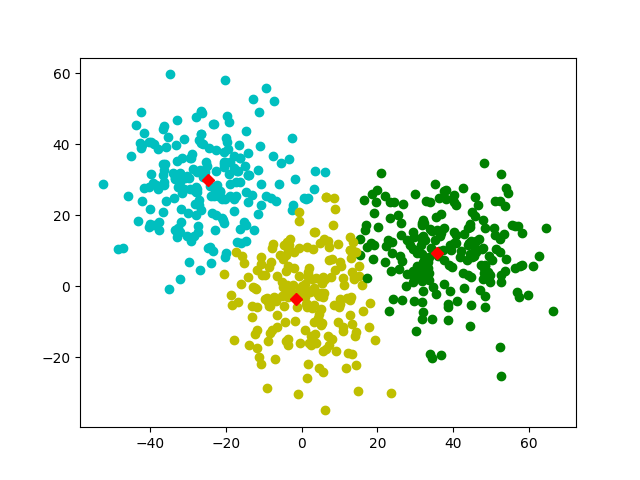
\includegraphics[width=0.65\textwidth]{figures/iteration4.png}}

\end{frame}

\begin{frame}
	\frametitle{Toward a K-means Algorithm}
	Iteration = 5
	\centerline{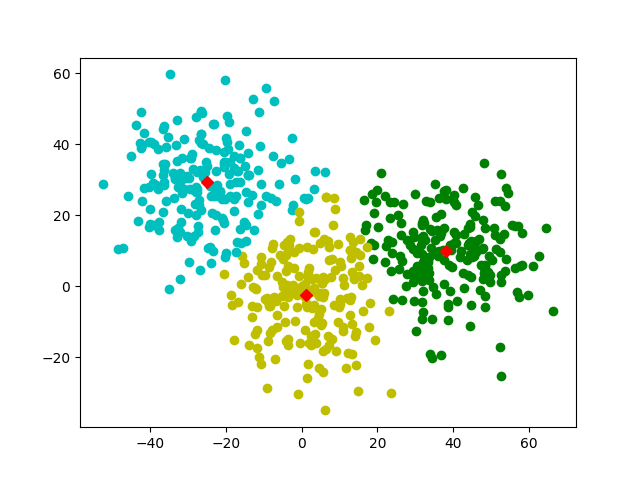
\includegraphics[width=0.65\textwidth]{figures/iteration5.png}}

\end{frame}

\begin{frame}
	\frametitle{Toward a K-means Algorithm}
	Iteration = 6
	\centerline{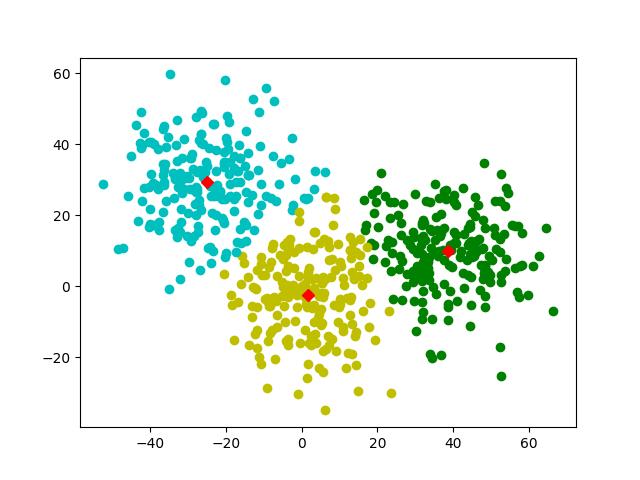
\includegraphics[width=0.65\textwidth]{figures/iteration6.png}}

\end{frame}

\begin{frame}
	\frametitle{Convergence of K-means}
	\begin{proof}
		During the course of the k-means algorithm, the cost monotonically decreases.
	\end{proof} \pause
	Let \ccb{$c_1^{(t)} \dots c_k^{(t)}, C_1^{(t)} \dots C_k^{(t)}$} denote the cetnroids and clusters at the start of $t^{th}$ iteration of K-means.
	\pause
	\par The first step of the iteration assigns each point to its nearest center, therefore:
	$$Cost(C_{1:k}^{(t+1)}, c_{1:k}^{(t)}) \leq Cost(C_{1:k}^{(t)}, c_{1:k}^{(t)})$$
	\pause
	On the second step, each cluster re-centered at its mean. By lemma above:
	$$Cost(C_{1:k}^{(t+1)}, c_{1:k}^{(t+1)}) \leq Cost(C_{1:k}^{(t+1)}, c_{1:k}^{(t)})$$

\end{frame}
%%//////////////////////////////////////////////////////////////////////////////////////////////%%
\begin{frame}
	\frametitle{Time Complexity}
	\begin{proof}
		Naive K-means algorithm's time complexity is \ccb{$O(kni)$}
	\end{proof} \pause
	In each iteration there are such steps:
	\begin{itemize}
		\item Distance calculation: To calculate the distance from a point to the centroid, we can use the squared Euclidean proximity function, which is thought to be $O(1)$
		\item Comparisons betweeen distances.
		\item Centroid calculation.
	\end{itemize}
\end{frame}

\begin{frame}
	\frametitle{Time Complexity}
	\begin{proof}
		Naive K-means algorithm's time complexity is \ccb{$O(kni)$}
	\end{proof}
	\par So the total number of operations in one iteration is:
	\begin{equation*}
		\begin{split}
			C &=  distance\ calculation + comparisons + centroids\ calculation\\
			& = k * n * O(1) + (k-1) * n * O(1) + k * n * O(1) \\
			& = O(kn)
		\end{split}
	\end{equation*}
	where k denotes the number of clusters, n denotes the count of data vectors and d denotes vector dimension.
	\par And the whole process takes $i$ iterations in total so the time complexity of K-means algorithm is \ccb{$O(kni)$}.
\end{frame}

\begin{frame}
	\frametitle{Drawback of K-means}

	

\end{frame}

\end{document}
